% Options for packages loaded elsewhere
\PassOptionsToPackage{unicode}{hyperref}
\PassOptionsToPackage{hyphens}{url}
%
\documentclass[
  ignorenonframetext,
]{beamer}
\usepackage{pgfpages}
\setbeamertemplate{caption}[numbered]
\setbeamertemplate{caption label separator}{: }
\setbeamercolor{caption name}{fg=normal text.fg}
\beamertemplatenavigationsymbolsempty
% Prevent slide breaks in the middle of a paragraph
\widowpenalties 1 10000
\raggedbottom
\setbeamertemplate{part page}{
  \centering
  \begin{beamercolorbox}[sep=16pt,center]{part title}
    \usebeamerfont{part title}\insertpart\par
  \end{beamercolorbox}
}
\setbeamertemplate{section page}{
  \centering
  \begin{beamercolorbox}[sep=12pt,center]{part title}
    \usebeamerfont{section title}\insertsection\par
  \end{beamercolorbox}
}
\setbeamertemplate{subsection page}{
  \centering
  \begin{beamercolorbox}[sep=8pt,center]{part title}
    \usebeamerfont{subsection title}\insertsubsection\par
  \end{beamercolorbox}
}
\AtBeginPart{
  \frame{\partpage}
}
\AtBeginSection{
  \ifbibliography
  \else
    \frame{\sectionpage}
  \fi
}
\AtBeginSubsection{
  \frame{\subsectionpage}
}
\usepackage{lmodern}
\usepackage{amssymb,amsmath}
\usepackage{ifxetex,ifluatex}
\ifnum 0\ifxetex 1\fi\ifluatex 1\fi=0 % if pdftex
  \usepackage[T1]{fontenc}
  \usepackage[utf8]{inputenc}
  \usepackage{textcomp} % provide euro and other symbols
\else % if luatex or xetex
  \usepackage{unicode-math}
  \defaultfontfeatures{Scale=MatchLowercase}
  \defaultfontfeatures[\rmfamily]{Ligatures=TeX,Scale=1}
\fi
% Use upquote if available, for straight quotes in verbatim environments
\IfFileExists{upquote.sty}{\usepackage{upquote}}{}
\IfFileExists{microtype.sty}{% use microtype if available
  \usepackage[]{microtype}
  \UseMicrotypeSet[protrusion]{basicmath} % disable protrusion for tt fonts
}{}
\makeatletter
\@ifundefined{KOMAClassName}{% if non-KOMA class
  \IfFileExists{parskip.sty}{%
    \usepackage{parskip}
  }{% else
    \setlength{\parindent}{0pt}
    \setlength{\parskip}{6pt plus 2pt minus 1pt}}
}{% if KOMA class
  \KOMAoptions{parskip=half}}
\makeatother
\usepackage{xcolor}
\IfFileExists{xurl.sty}{\usepackage{xurl}}{} % add URL line breaks if available
\IfFileExists{bookmark.sty}{\usepackage{bookmark}}{\usepackage{hyperref}}
\hypersetup{
  pdftitle={Beamer Slide Element Templates},
  hidelinks,
  pdfcreator={LaTeX via pandoc}}
\urlstyle{same} % disable monospaced font for URLs
\newif\ifbibliography
\usepackage{graphicx,grffile}
\makeatletter
\def\maxwidth{\ifdim\Gin@nat@width>\linewidth\linewidth\else\Gin@nat@width\fi}
\def\maxheight{\ifdim\Gin@nat@height>\textheight\textheight\else\Gin@nat@height\fi}
\makeatother
% Scale images if necessary, so that they will not overflow the page
% margins by default, and it is still possible to overwrite the defaults
% using explicit options in \includegraphics[width, height, ...]{}
\setkeys{Gin}{width=\maxwidth,height=\maxheight,keepaspectratio}
% Set default figure placement to htbp
\makeatletter
\def\fps@figure{htbp}
\makeatother
\setlength{\emergencystretch}{3em} % prevent overfull lines
\providecommand{\tightlist}{%
  \setlength{\itemsep}{0pt}\setlength{\parskip}{0pt}}
\setcounter{secnumdepth}{-\maxdimen} % remove section numbering
\usepackage{multicol}

\title{Beamer Slide Element Templates}
\author{}
\date{\vspace{-2.5em}}

\begin{document}
\frame{\titlepage}

\begin{frame}[fragile]{iClicker Answer List Code}
\protect\hypertarget{iclicker-answer-list-code}{}

\begin{verbatim}
\begin{enumerate}[A]
  \item Q1
  \item Q2
  \item Q3
  \item Q4
  \item Q5
\end{enumerate}
\end{verbatim}

\end{frame}

\begin{frame}{iClicker Answer List}
\protect\hypertarget{iclicker-answer-list}{}

\begin{enumerate}[A]
\item Q1
\item Q2
\item Q3
\item Q4
\item Q5
\end{enumerate}

\end{frame}

\begin{frame}[fragile]{iClicker Logo Code}
\protect\hypertarget{iclicker-logo-code}{}

\begin{verbatim}
\begin{multicols}{2}
\null \vfill
\vfill \null
\columnbreak
\includegraphics[width = 0.35\textwidth]{{`r here(img_dir, "iClicker_logo.png")`}}
\end{multicols}
\end{verbatim}

\end{frame}

\begin{frame}{iClicker Logo}
\protect\hypertarget{iclicker-logo}{}

\begin{multicols}{2}
\null \vfill
\vfill \null
\columnbreak

\includegraphics[width = 0.35\textwidth]{C:/git/NRC290B/slides/slide_images/iClicker_logo.png}
\end{multicols}

\end{frame}

\begin{frame}[fragile]{Image File Code}
\protect\hypertarget{image-file-code}{}

\begin{verbatim}
\begin{center}
    \includegraphics[width = 0.88\textwidth]
        {`r here(img_dir, "question_mark_green.png")`}
\end{center}
\end{verbatim}

\end{frame}

\begin{frame}{Image File}
\protect\hypertarget{image-file}{}

\textbackslash begin\{center\} \textbackslash includegraphics{[}width =
0.88\textwidth{]}
\{C:/git/NRC290B/slides/slide\_images/question\_mark\_green.png\}
\textbackslash end\{center\}

\end{frame}

\begin{frame}{R Figure I}
\protect\hypertarget{r-figure-i}{}

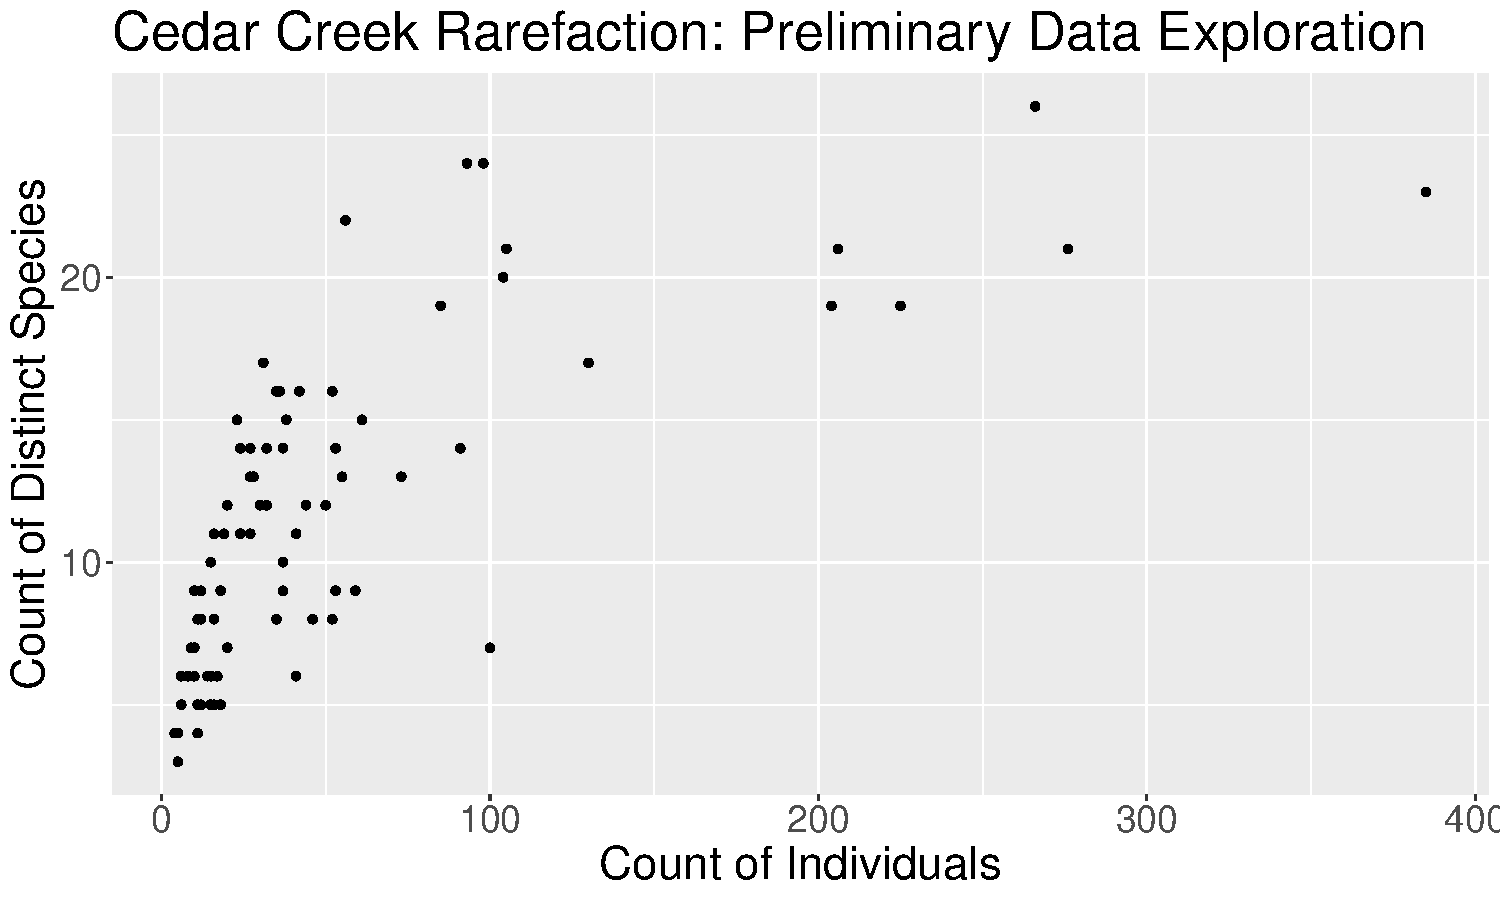
\includegraphics{slide_element_templates_files/figure-beamer/r figure fixed aspect-1.pdf}

\end{frame}

\begin{frame}{R Figure II}
\protect\hypertarget{r-figure-ii}{}

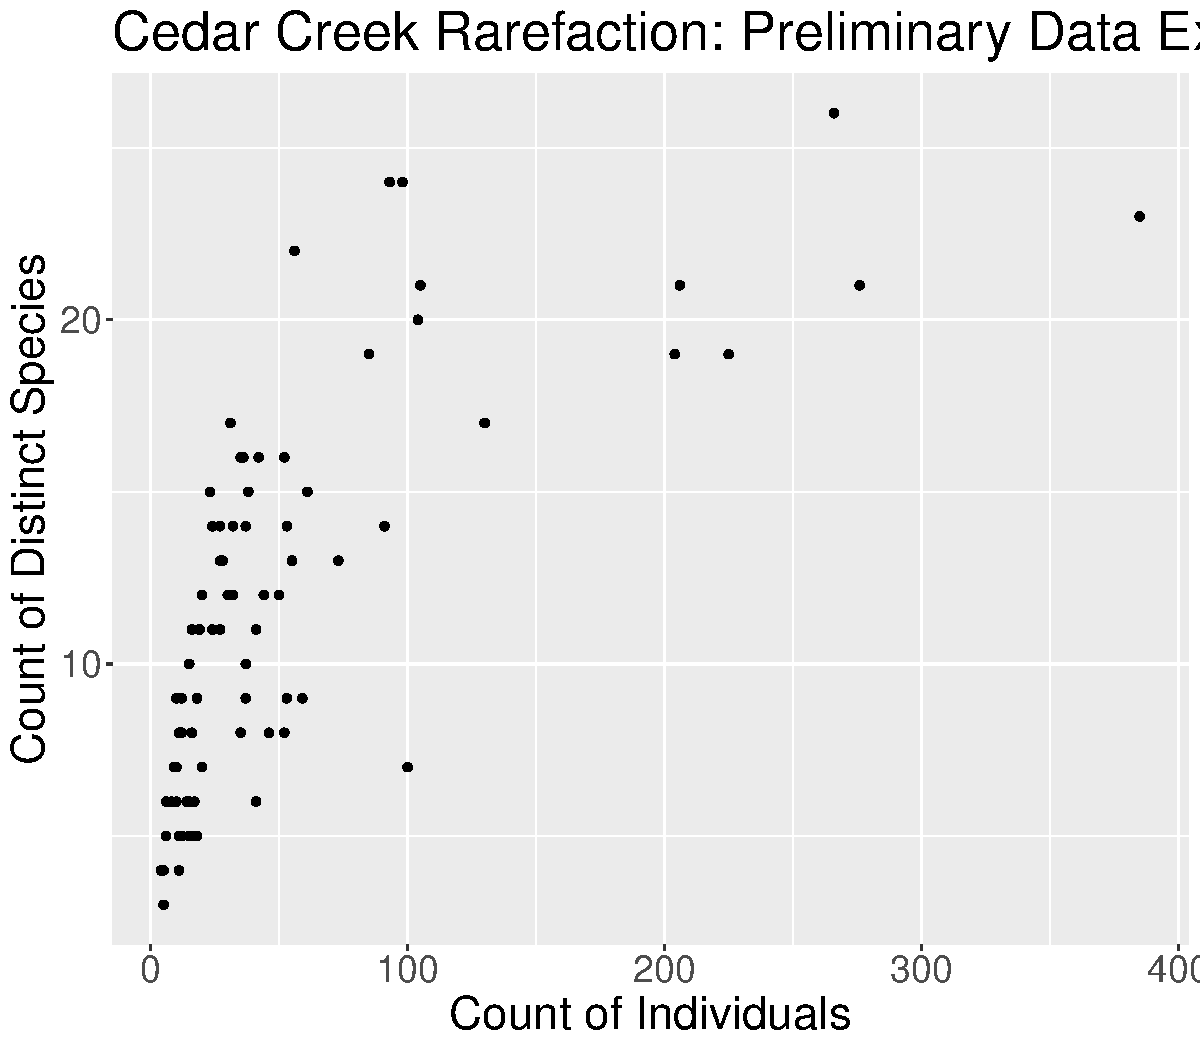
\includegraphics{slide_element_templates_files/figure-beamer/r figure set height and width-1.pdf}

\end{frame}

\begin{frame}{Nested List}
\protect\hypertarget{nested-list}{}

The data (i.e.~the variables):

\begin{enumerate}
  \item Response Variable
  \begin{enumerate}
    \item the variable of interest
  \end{enumerate}
  \item Explanatory Variables
  \begin{enumerate}
    \item predictor
  \end{enumerate}
\end{enumerate}

\end{frame}

\begin{frame}[fragile]{Nested List Code}
\protect\hypertarget{nested-list-code}{}

\begin{verbatim}
\begin{enumerate}
  \item Response Variable
  \begin{enumerate}
    \item the variable of interest
  \end{enumerate}
  \item Explanatory Variables
  \begin{enumerate}
    \item predictor
  \end{enumerate}
\end{enumerate}
\end{verbatim}

\end{frame}

\begin{frame}[fragile]{Equations Code}
\protect\hypertarget{equations-code}{}

\begin{verbatim}
\begin{equation}
   \label{eq:example-equation}
   y = mx + b
\end{equation}

\begin{equation}
   \label{eq:example-equation}
   y_{i} = 
   \alpha + 
   \beta_{1} \times 
   x_{i1} + 
   \beta_{2} \times 
   x_{i2} + 
   \epsilon
\end{equation}
\end{verbatim}

\end{frame}

\begin{frame}{Equations}
\protect\hypertarget{equations}{}

\begin{equation}
   \label{eq:example-equation}
   y = mx + b
\end{equation}

\begin{equation}
   \label{eq:example-equation}
   y_{i} = \alpha + \beta_{1} \times x_{i1} + \beta_{2} \times x_{i2} + \epsilon
\end{equation}

\end{frame}

\begin{frame}[fragile]{Figure and Footnote Code}
\protect\hypertarget{figure-and-footnote-code}{}

\begin{verbatim}
\begin{center}
    \includegraphics[width = 0.35\textwidth]
       {`r here(img_dir, "iClicker_logo.png")`}
\end{center}

\footnotetext[1]
   {Figure 4.3 in Fletcher and Fortin, 2018}
\end{verbatim}

\end{frame}

\begin{frame}{Figure and Footnote}
\protect\hypertarget{figure-and-footnote}{}

\begin{center}

\includegraphics[width = 0.35\textwidth]{C:/git/NRC290B/slides/slide_images/iClicker_logo.png}
\end{center}

\footnotetext[1]{Figure 4.3 in Fletcher and Fortin, 2018}

\end{frame}

\end{document}
